% % % % % % % % % % % % % % % % % % % % % % % % % % % % % % % % 
% BSc Physics Dissertation
% % % % % % % % % % % % % % % % % % % % % % % % % % % % % % % %
\documentclass[twoside, fontsize=12pt,
     bibliography=totoc, % Include bibliography in contents
     listof=totoc, % Include lists of figures and tables in contents
     index=totoc, % Include index in contents
     onehalfspacing %  or doublespacing
    %,openright
]{_MScDiss2017_cls}

%\usepackage{txfonts,epsfig}
\usepackage[labelfont=footnotesize,textfont=footnotesize]{caption}   
\usepackage{_twoopt}
\usepackage{url}
\usepackage[colorlinks,citecolor=blue,linkcolor=blue,urlcolor=blue,hyperfootnotes=false,linktocpage,breaklinks=true]{hyperref}
%\usepackage{breakurl}
\usepackage[]{_MScDiss_sty}
%\usepackage{chngcntr}
%\counterwithout{footnote}{chapter}
\usepackage{listings}
\usepackage{fontspec-xetex}
\usepackage{xcolor}
\usepackage{float}

\newfloat{lstfloat}{htbp}{lop}
\floatname{lstfloat}{Listing}
%\def\lstfloatautorefname{Listing}
%\setmonofont{Courier}
%% these macros turn citations into ADS clickers in dvi, pdf, html output
%% (EDP Sciences improved them in December 2012 to work also with pdflatex)
\bibpunct{(}{)}{;}{a}{}{,}    %% natbib cite format used by A&A and ApJ
\makeatletter
 \newcommandtwoopt{\citeads}[3][][]{\href{http://adsabs.harvard.edu/abs/#3}%
   {\def\hyper@linkstart##1##2{}%
    \let\hyper@linkend\@empty\citealp[#1][#2]{#3}}}    %% Rutten, 2000
 \newcommandtwoopt{\citepads}[3][][]{\href{http://adsabs.harvard.edu/abs/#3}%
   {\def\hyper@linkstart##1##2{}%
    \let\hyper@linkend\@empty\citep[#1][#2]{#3}}}      %% (Rutten 2000)
 \newcommandtwoopt{\citetads}[3][][]{\href{http://adsabs.harvard.edu/abs/#3}%
   {\def\hyper@linkstart##1##2{}%
    \let\hyper@linkend\@empty\citet[#1][#2]{#3}}}      %% Rutten (2000)
 \newcommandtwoopt{\citeyearads}[3][][]%
   {\href{http://adsabs.harvard.edu/abs/#3}%
   {\def\hyper@linkstart##1##2{}%
    \let\hyper@linkend\@empty\citeyear[#1][#2]{#3}}}   %% 2000
\makeatother

\declaration{I hereby certify that this Dissertation, has been written by me at the School of Physics and Astronomy, Queen Mary University of London, that all material in this dissertation which is not my own work has been properly acknowledged, and  that it has not been submitted in any previous application for a higher degree.} 

%--Put your information between here----%
\title{The Effects of Energy Densities on the CMB Power Spectrum}
\author{Daniil Dolgich (150066826)}
\supervisor{Prof. Teppei Katori}
\date{\today}
%\date{July 2019} 
\acknowledgements{I'd like to give my appreciation to Prof. Teppei Katori for supervising my project even though it was outside of his comfort zone. There was a lot of mutual learning that made this all the more valuable. I would also like to thank him for his patience and support in regards to my health and well-being.
\paragraph{}
Consultation by Dr. Alkistis Pourtsidou was very helpful in kick-starting my understanding regarding the topics in this project. Her passion for her field inspired me to pursue this topic.
\paragraph{}
Many thanks as well to Harvey Abraham-Green and Leonie Dos Santos for offering their time and support when it was needed most.
\paragraph{}
Finally, a big thank you to my parents.
}
\newpage % to ensure page 1 starts on front of a page rather than back
%%---and here------%

\begin{document}
\pagenumbering{roman}
\setcounter{tocdepth}{5}

\maketitle
\abstract{We studied the Cosmic Microwave Background radiation (CMB) in order to better understand the lesser studied portions of the CMB power spectrum. To facilitate this, I created my own CMB simulator with Python 2.7, using Jupyter Notebook as the compiler and GitHub to store my work.
\paragraph{}
I used this simulator to demonstrate the effects that different values of the energy density for baryonic matter ($\Omega$\textsubscript{b}), dark matter ($\Omega$\textsubscript{c}), and neutrinos ($\Omega$\textsubscript{$\nu$}) have on the CMB power spectrum, and what observations could be made regarding the outcomes.
\paragraph{}
I found that altering the values of $\Omega$\textsubscript{c} caused the first peak of the CMB spectrum to greatly increase in amplitude and width, whilst smoothing out the rest of the power spectrum past that point. It also moved the maximum of the peak from $\ell$$\approx$200 to $\ell$$\approx$300, resulting in a huge and significant temperature fluctuation of $\sim$0.1$\mu$K.
\paragraph{}
Altering the values of $\Omega$\textsubscript{c} caused the overall amplitude of the spectrum to go down, but maintained well defined peaks and did not shift the relative x-axis position of the peaks in any direction.
\paragraph{}
Increasing the value of $\Omega$\textsubscript{$\nu$} caused an overall smoothing of the power spectrum, as well as a large reduction in the amplitudes of the peaks, and a slight shift of the first peak maximum to the left.
\paragraph{}
We saw that having a higher ratio of baryonic matter would result in a huge increase to the CMB anisotropy, and that a high neutrino energy density creates more "empty space" (space that is occupied by extremely unreactive neutrinos instead of any other particle). These would change our perception of when important cosmological events occurred, and would also affect large cosmological bodies such as galaxy clusters.

}
\tableofcontents % generates Table of Contents
\listoffigures % generates List of figures
\lstlistoflistings % generates List of listings

\newpage% to flush out last roman numeral
\cleardoublepage
\pagenumbering{arabic}% Set arabic page numbers now that dissertation proper is starting.

% rather than having a very long file you can Input files for each chapter/section here using 
% \input{relative-path-to-file} or just put the files in the same directory as this file.

%Chapter
\chapter{Introduction}
The Cosmic Microwave Background radiation (CMB) is electromagnetic radiation (EM) from the time of the Big Bang. Over the course of around 13 billion years, the CMB has been red-shifted to longer wavelengths due to the persisting expansion of the universe. As such, it has cooled dramatically from its initial state about 300,000 years after the Big Bang. The exact nature of the origins of the CMB and the Big Bang theory are beyond the scope of this project; however, the important part of this is that the CMB is about 2.7 Kelvin above absolute zero. \cite{PostgradCMB}

\paragraph{}

At cosmological scales, about 100 giga parsecs (Gpc), the universe may be taken to be homogeneous and isotropic. In other words, the universe is the same in all locations, and in all directions. The CMB is therefore also considered to be both of these things when looking at such immense scales. However, this is not quite the case for the CMB.

\paragraph{}

\begin{figure}
	\begin{center}
	\includegraphics[width=\textwidth]{WMAP-map}
	\caption{WMAP CMB Anisotropy Photo. Note the speckled appearance as a result of many hot and cold zones. \cite{UCLA}}
	\label{wmapcmb}
	\end{center}
\end{figure}

One can see in the image of the CMB taken by the Planck satellite (figure \ref{wmapcmb} that it's quite the opposite in fact. There are many zones of differing temperatures. The CMB is not wholly isotropic and this image shows that very clearly. These fluctuations are incredibly small, within the order of micro-Kelvin, and are collectively known as anisotropy. \cite{UCLA}

\paragraph{}

The way to describe the CMB anisotropy is with spherical harmonics. \cite{Berkeley} As such, the CMB power spectrum is actually an angular power spectrum. Under the model of Inflation, these temperature fluctuations are Gaussian, and the variance is given by $C$\textsubscript{$\ell$}. $\ell$ in this instance is the multipole moment. Different values of $\ell$ represent a given angle in the sky, and can be thought of as angular frequency for the temperature fluctuations, with higher values of $\ell$ corresponding to smaller angles. Essentially, the value of $\ell$ can be thought of as "how many opposite zones are there", the simplest of which is a dipole, in which there are two zones, opposites of each other, just like a bar magnet. As you increase the number of zones, the number of poles will also increase. This is essentially what the CMB power spectrum represents; at higher values of $\ell$, there are many many more zones being observed simultaneously. This can be seen in figure \ref{cmball}.

\begin{figure}
	\begin{center}
	\includegraphics[width=\textwidth]{cu-1000-031.pdf}
	\caption{Cumulative image of the sky, featuring a multipole $\ell$ value of 260. This closely resembles the pattern in figure \ref{wmapcmb}, and the fluctuations are also not equally distributed. You can also see the corresponding relative position on the CMB power spectrum plot in the top left corner. \cite{Pryke}}
	\label{cmball}
	\end{center}
\end{figure}

\paragraph{}

We can see how the plots of the multipole moment against the temperature fluctuations in $\mu$$K$$^2$ results in the CMB power spectrum. The three characteristic peaks correspond to the curvature of the universe, the baryon density, and the cold dark matter density, though the exact reasons why are beyond the scope of this research.

\paragraph{}

There are three commonly considered energy densities used to construct the CMB power spectrum: $\Omega$\textsubscript{b} which denotes normal baryonic matter, $\Omega$\textsubscript{c} denotes cold dark matter, and $\Omega$\textsubscript{$\Lambda$} denotes dark energy. This however neglects another energy density value, specifically, $\Omega$\textsubscript{$\nu$}, the energy density of neutrinos. 

\paragraph{}

With this in mind, I decided to create my own CMB simulator to see exactly how different values for these energy densities affects the power spectrum, and how the overall composition of the universe would change.

\chapter{Methodology}

\section{Preliminary research}
Before I could begin, I had to first familiarise myself with the precise meanings of each element of the CMB power spectrum and how anisotropy was the underlying aspect.

\paragraph{}

I found online, two simulators of the CMB, one simplistic and the other incredibly in-depth. \cite{SimpleCMB} The simplistic one was similar to what I had planned to make myself: a simulator that allows changing of variables and instantly outputs the new graph. The second simulator did not have this feature but had a large selection of variables to tweak. \cite{LambdaToolsCMBSimulator}

\paragraph{}

The second simulator, upon completion of the simulation, would also provide a data file in which were contained the multipole moment values ranging from 2 to 2200, as well as the temperature fluctuations for the different versions of the CMB spectrums. The one I was concerned with was the temperature angular power spectrum (TT). I used this file as the input for all the base variables in my simulator. I also looked at the values presented  for the temperature-polarisation cross-power spectrum (TE) and the polarised spectrum (EE), and decided to also simulate these graphs for the purposes of comparison; to see whether they get affected the same way as my baseline TT graph. There was no intent to delve deeper into the effects of the polarisation at this time.

\section{Making the simulator}

The language of choice was Python 2.7. Using this I was able to start work on constructing the simulator.

\paragraph{}

I chose to use Jupyter Notebook \cite{JupyterNotebook} as my platform to code on, and a GitHub repository \cite{Github} to commit and push my work to. The first step was to gather all the necessary data, as well as import all the necessary packages. 

\lstset{
	language=Python,
	frame=lines,
	rulecolor=\color{magenta},
	numbers=left,
	numbersep=10pt,
	basicstyle=\ttfamily\small,
	numberstyle=\ttfamily\small,
	breaklines=true,
	keywordstyle=\bfseries\color{teal},
	identifierstyle=\color{blue},
	stringstyle=\color{red},
	commentstyle=\itshape\color{lime},
	basewidth=0.55em,
}
\begin{lstfloat}
\begin{lstlisting}[caption={Setting up}, captionpos=b]
import camb
import matplotlib
import matplotlib.pyplot as plt
import numpy as np
from ipywidgets import interact
import ipywidgets as widgets

params = camb.read_ini('camb_interface/camb_params.ini')
\end{lstlisting}
\end{lstfloat}

\paragraph{}
This imported the primary packages that I needed in order to make the graph and have it actually function. CAMB is Code for Anisotropies in the Microwave Background and is used for calculating many things within cosmology \cite{PythonCAMB}. It just so happens to also use Python as the main code. Matplot was necessary to have a way to draw the graph. NumPy was used to manipulate the data from CAMB and pass it on to Matplot to use in the formation of the graph \cite{numpy}. IPyWidgets was to create the interactive controls to vary the values of the graph and output the changes in real time \cite{widgets}.

\paragraph{}

The next step was to create a function that would be called and "interacted" with. I defined this first run as "camb\_plot\_tt", and also defined the values that I would have available to change; each of the "om\_h2" represent their respective energy densities, with om standing for $\Omega$, h2 being Planck's constant squared ($h$$^2$), and with the letter corresponding to its respective object: b for baryons, c for dark matter, nu for neutrinos.

\paragraph{}

\begin{lstfloat}
\begin{lstlisting}[caption={Initialising the first plot}, captionpos=b]
%matplotlib inline
def camb_plot_tt(ombh2, omch2, omnuh2):
    params.ombh2 = ombh2
    params.omch2 = omch2
    params.omnuh2 = omnuh2
    results = camb.get_results(params)

    unlensed = results.get_cmb_unlensed_scalar_array_dict(lmax=2200, CMB_unit='muK')

    tt = unlensed['TxT']

    fig, ax = plt.subplots()
    tt = np.delete(tt, [0, 1])
    ax.plot(tt, linewidth=1)
    ax.set_xlim([None, 2500])
    ax.set_ylim([None, 7000])
    ax.set(xlabel='Multipole Moment (l)', ylabel='CMB_Unit (uK^2)', title='Cl TT CMB Power Spectrum')
    fig.savefig("Cl-TT-vs-l.pdf")
    plt.show()

\end{lstlisting}
\end{lstfloat}

%\paragraph{}

Here I set the initial values for each of the three variables as the defaults present within the CAMB data. By assigning variables in Python, I was able to save some time and avoid having to rewrite too much. 'TxT' was taken from the array and contained all the data points for plotting the TT CAMB graph. Once I assigned reasonable limits for the axes and added a handy feature to save the future plot as a .pdf file, I moved on to figuring out how to create the interactive sliders for the three variables.

%\paragraph{}


\begin{lstfloat}
\begin{lstlisting}[caption={Creating the first plot}, captionpos=b]
params = camb.read_ini('camb_interface/camb_params.ini')
interact(camb_plot_tt,
         ombh2=widgets.FloatSlider(value=params.ombh2, min=0, max=1, step=0.001, readout_format='.5f'),
         omch2=widgets.FloatSlider(value=params.omch2, min=0, max=1, step=0.001, readout_format='.5f'),
         omnuh2=widgets.FloatSlider(value=params.omnuh2, min=0, max=1, step=0.001, readout_format='.5f'));
\end{lstlisting}
\end{lstfloat}

\paragraph{}

By using the floatsliders present in iPywidgets, I was able to assign the minimum and maximum values for the variables and also assign an appropriate step value of 0.001. The readout format was chosen specifically to avoid visually truncating the value of the $\Omega$\textsubscript{$\nu$} value, as it's very small at default (0.00064).

\paragraph{}

Running these three cells in sequence created the graph you see in figure \ref{fig:TT}, which is a near perfect match to the plot I saw during my initial research. With this now functioning program, I set about checking what happens when I change the values of the variables.

\paragraph{}

Initially however, I discovered a flaw in my programming. Because I had constrained $\Omega$\textsubscript{$\Lambda$}, this meant that its value was completely fixed; the total energy density $\Omega$\textsubscript{total} has to equal 1 because it is comprised of ratios, but in my simulator, you can go beyond that and end up breaking the simulator. This same error occurs if variables are changed too quickly.

\paragraph{}

Regardless, I was able to get a working version of the simulator, and decided to plot the EE and TE values to see that they also matched the ones seen on the Lambda website (see figure \ref{ogcmb}).

\label{sec:template}

\begin{figure}
	\begin{center}
	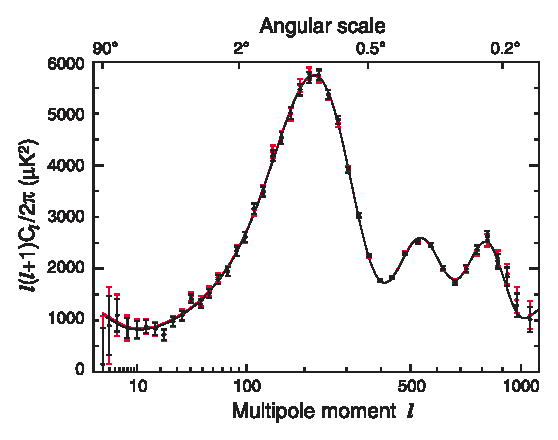
\includegraphics[width=\textwidth]{gh9-f02.eps}
	\caption{The WMAP nine-year power spectrum to which I was comparing my plot. Notice how the maximum peak at around $\ell$$\approx$200 is also around 1$^\circ$ on the angular scale. \cite{LambdaTools}}
	\label{ogcmb}
	\end{center}
\end{figure}

\begin{figure}[t]
  \begin{center}
  \includegraphics{2Cl-TT-vs-l.pdf}
  \caption{My plot of the Scalar Non-lensed CMB Power Spectrum TT} 
  \label{fig:TT}
  \end{center}
\end{figure}

\chapter{Results}

I chose to alter each variable individually, one at a time, in order to be sure that that specific variable was responsible for the change in the graph.

\paragraph{}

My predictions were mainly these:
\paragraph{}
Increasing $\Omega$\textsubscript{b} would result in the graph becoming more "smeared", causing the peaks to shrink and become less defined, as more regular matter would mean there are many more minute interactions occurring and thus muddying the spectrum.
\paragraph{}
Increasing $\Omega$\textsubscript{c} would result in the graph growing in intensity, as dark matter is much more massive than regular matter, and so I expect the fluctuations to also increase alongside the increase in dark matter.
\paragraph{}
Increasing $\Omega$\textsubscript{$\nu$} would also result in a smearing of the graph, and a reduction in the amplitudes, but not for the same reasons as with baryonic matter; neutrinos are incredibly light and interact with very little, meaning that an increase in neutrinos would result in there being less room within each measured multipole for dark  matter or baryonic matter. Essentially, neutrinos would add what could be thought of as "empty space" between particles that would otherwise interact.

\paragraph{}

The most notable thing is that past a certain point, increases in value for each variable have less and less effect on the graph. There appears to be a point at which the graph seemingly stops changing. I assume this is due to my constrained $\Omega$\textsubscript{$\Lambda$} not allowing any further changes to occur. However, the immediate effects are visible from even very minute changes to each variable.

\begin{figure}[t]
	\begin{center}
	\includegraphics{3Cl-TT-vs-l}
	\caption{TT Spectrum with biased $\Omega$\textsubscript{b}. The first peak maximum skyrockets beyond the y-axis limit while the other peaks become smeared and start to homogenise.}
	\label{fig:bbias}
	\end{center}
\end{figure}

\paragraph{}

Strangely, for baryonic matter, my prediction was only half wrong. In figure \ref{fig:bbias} the amplitudes of the second and third peaks became heavily smeared, as expected, but the first peak amplitude rose well past the y-limit I had assigned in my code. I cannot say as to why that is the case. Interestingly, the dipole peak seems to have also shifted to around $\ell$$\approx$300, suggesting that the corresponding angle has also gone down below 1$^\circ$.

\paragraph{}

\begin{figure}
	\begin{center}
	\includegraphics{4Cl-TT-vs-l}
	\caption{TT Spectrum with biased $\Omega$\textsubscript{c}. Lowered total amplitude but peaks are still well defined and the position of the peak maximum has remained the same.}
	\label{fig:cbias}
	\end{center}
\end{figure}

For dark matter, this test also went against my prediction entirely. Figure \ref{fig:cbias} shows that increasing the dark matter actually greatly lowered the amplitudes of all the peaks. However, and quite notably, it has not smeared the graph like the baryonic change. The peaks are still quite well defined, and only their amplitudes have shrunk. This suggests that this ends up greatly reducing the anisotropy, and thus the temperature fluctuations. Additionally, the two most well-defined peaks remain at $\ell$$\approx$200 and the third peak which we know from our preliminary research to be the dark matter peak; considering it is the amount of dark matter we have increased in this simulation, this is a very logical outcome.

\begin{figure}
	\begin{center}
	\includegraphics{5Cl-TT-vs-l}
	\caption{TT Spectrum with biased $\Omega$\textsubscript{$\nu$}. Huge decrease in overall amplitude, in addition to lots of smoothing of the line, suggesting increased homogeneity due to the increased amount of neutrinos in this particular simulation.}
	\label{fig:vbias}
	\end{center}
\end{figure}

\paragraph{}

Figure \ref{fig:vbias} shows the neutrino biased simulation to be quite similar in results to the the dark matter simulation initially, however, the peaks are not as well defined, indicating that the graph has indeed been smeared and smoothed, matching my initial prediction. This was the particular simulation I was interested in doing, as it had been absent from the two simulators mentioned in the introduction to this document, and it shows that neutrino energy density is as impactful and important to the composition of the universe as the three most considered values for baryonic matter, dark matter and dark energy.

\paragraph{}

Comparing the three graphs shows that biasing $\Omega$\textsubscript{b} creates the most noticeable change, and more specifically, that it hugely increases the temperature fluctuations at the lower values of $\ell$, as well as moving the maximum of the largest first peak to be at a slightly higher value of $\ell$ compared to the other two graphs. In figure \ref{fig:bbias}, the first peak exceeds the maximum limit on the graph; I predict it reaches at least 10000$\mu$$K$$^2$, meaning that the real temperature fluctuation is $\sim$0.1$\mu$$K$, which is a very significant anisotropy. 
\paragraph{}
One could infer what sort of consequences may arise on a universal scale as a result of this, such as how it would affect the rate of expansion, as well as the percentage of accompanying dark matter, dark energy, and neutrinos. Certain other phenomenon such as galaxy cluster lensing would also get affected by fluctuating rates of dark matter, and the size of the galaxy clusters would also change in accordance with the amount of dark matter present in the universe.

%\paragraph{}



\chapter{Conclusions}

By matching the simulations to observed results, we can figure out precise, allowed values for specific objects and phenomena. Here, most notably, we can see how big of an impact the energy density of neutrinos has on the CMB power spectrum, and indeed, also confirms that neutrinos are not massless.

\paragraph{}

This also means that neutrinos must have a maximum allowed mass. Since energy is related to mass, if their energy density was higher, their mass would also need to be higher. As seen from the simulation, a higher amount of neutrinos would likely start to prevent further reactions from taking place.

\paragraph{}

Additionally, the dark matter result was not expected and shows that an increase in dark matter would result in much lower temperature fluctuations across the CMB, meaning that in turn, the universe could be considered homogeneous and isotropic at slightly smaller scales than what are used now.

\paragraph{}

These rudimentary simulations have shown the possible effects on CMB anisotropy, and subsequently on the distribution of different types of matter within the universe. Though these are mostly hypothetical scenarios, they can be useful to help us to predict the behaviour of certain particles, or indeed on larger scales such as galaxy clusters and possibly even black holes, though more research would need to be done on that particular case.

\paragraph{}

There is much more that can be factored in that was beyond the scope of this project; the lensing effect along with the alternate forms of the CMB spectrum in the temperature-polarisation cross-spectrum TE, and the polarised spectrum EE. Exploring this further could yield some very interesting results.

%%BIBLIOGRAPHY SECTION
\begin{singlespace}% Start single space for bibliography
\bibliographystyle{_abbrvnat_jpe}    
\bibliography{Dolgich.bib} %makes BIBLIOGRAPHY from the listed bib files  
\end{singlespace}

\end{document}
